\newpage
\section{Symmetric abstractions}\label{symmetric-abstractions}

% symmetry is cool
Symmetry is a concept from pure mathematics, which has found major success in physics (for example, \href{https://en.wikipedia.org/wiki/Noether%27s_theorem}{see Noether's theorem}).
Symmetry has also had success in machine learning. For example, the notion has led to;
data augmentation strategies \cite{Simard2003},
understanding of convolutional neural networks \cite{Cohen2017}, and a definition of disentanglement \cite{Higgins2018}.
We are interested in using symmetry to build abstractions for RL. But first, what do we mean by symmetry?

% also, to disentanglement
% % Connection to causal hierarchy. Cite Pearl. Association, intervention, counterfactuals.
% Also recently noted by \cite{Caselles-Dupre2019}, ... where they assume that
% the group actions are the actions of the RL environment.
% This doesn't really make sense. Also, will miss many symmetries like ???

% occam's razor
% Occam's razor is a core idea behind much of statistics, ML and science. Simple
% hypotheses should be preferred as the are more likely to be right.


\subsubsection{Definition}

We say that an object is symmetric if it has 'group' structure.

A group is a set, $G$ (\textit{say the set of rotations, $\{0, 90, 180, 270\}$}),
and an operation $\circ$ that combines any two elements $a$ and $b$ to form
another element (\textit{rot $90$ composed with rot $180$ is rot $270$, or} $a \circ b = a + b \;\text{mod} 360$).
To qualify as a group, the set and operation, $(G, \circ)$, must satisfy four requirements;

\begin{itemize}
	\tightlist
	\item \textbf{Closure:} For all $a, b \in G$, the result of the operation $a \circ b$ is also in $G$. (\textit{every composition of two rotations, must also be a rotation})
	\item \textbf{Associativity:} For all $a,b,c \in G$, $(a\circ b) \circ c = a\circ (b\circ c)$.
	\item \textbf{Identity element:} There exists and element $e\in G$ such that, for every element $a\in G$, the equation $e\circ a = a\circ e = a$ holds. (\textit{there must exist a rotation that doesn't rotate})
	\item \textbf{Inverse element:} For each $a \in G$, there exists an element $b \in G$, commonly denoted $a^{−1}$, such that $a \circ b = b \circ a = e$. (\textit{we must be able to undo any rotation})
\end{itemize}



\begin{displayquote}
\textsl{How can symmetries be used to build abstractions?}
\end{displayquote}

We can use a group structure to define a similarity (aka an equivalence relation),
$a \sim_G b$ iff $\exists g \in G: a = g \circ b$. For some examples of symmetries within RL see \ref{game-invariants}.
Therefore, we can use this notion of similarity, as we did in \ref{C:abstraction}, to construct abstractions.

% How does knowing the specific structure of the similarities help?   !!!!!
% If we are just going to group them together?

\subsection{A symmetric inductive bias}

% Following our insights from \ref{symmetry} and \ref{???}.
% This is about generalising using an inductive bias towards symmetry.

In \ref{infer-similarity} we considered using similarities
to build an abstraction. But, learning pairwise similarities does not give
you the ability to generalise\footnotemark. To generalise you need (accurate) priors \cite{Wolpert1996}.

\footnotetext{Knowing that $a$ and $b$ are similar tells you nothing about $c$ and / or $d$.}

Existing approaches to estimating similarity can generalise if the (measure of) similarity encodes priors.
For example:
If our measure of similarity is parameterised as a CNN, then the CNN implicitly encodes a preference for continuous and local functions\cite{Yann1995}.
If our measure of similarity is trained using SGD, SGD implicitly encodes a preference for low rank solutions \cite{Gunasekar2017}.

In this section we explore how to construct a prior that says:

\begin{displayquote}
	\textsl{We believe that the problems we are given will have group structure.}
\end{displayquote}

This symmetric prior allows us to impose abstract structure on potential similarities, without specifying
the 'details' of these similarities.

% \subsubsection{Closedness and generalisation}
%
% The key property we are interested in is the \textit{closure}.
% By requiring the
%
%  Symmetry is a stricter notion of similarity, it requires ...?
%  % If $x, x' \in X$ are symmetric, then there must exist $f$ such that $f(x) = x'$.
%  % Where, $(X, f)$ must satisfy the group axioms, (closure, associativity, identity, inverse).
%
%  Two $x, x'$ are considered symmetric if $\exists g\in G$

% - What about symmetries that are products of subgroups? $S = Z_2 \times Z_3$? Are they easier to infer?
% - Within the same $n$. Is there a notion of more or less complex group structures??
% - Need to show that NNs dont have the right symmetric inductive bias. They dont generalise. !!!

\subsection{A measure of symmetry}\label{measure-symmetry}

\begin{displayquote}
	\textsl{To build this prior, we need to be able to measure symmetries.}
\end{displayquote}

We need to construct a measure of symmetry, $S: X \to \mathbb [0, 1]$, that returns higher values for 'more' symmetric objects.
We can then use this measure to bias a learner towards more symmetric guesses (see \ref{thompson-sampling}).

Given an object, $x \in X$, we want to know, how symmetric is that object?
% This would allow us to consider alterative possibilities, such as $y \in X$, and say that we prefer $x$ to $y$ because $x$ is more symmetric.
But, what makes something more or less symmetric?
We define the amount of symmetry to be: the order \footnotemark of the largest group that $x$ is invariant to.

\footnotetext{The order of a group is defined as the cardinality of the set of group elements, which is written $|G|$.}

For example, $x_{ab} = [a,a,b,b]$ should be considered more symmetric than $x_{abc} = [a,a,b,c]$ because,
$x_{ab}$ is invariant to actions\footnotemark of $S_2 \times S_2$, while $x_{abc}$ is (only) invariant to actions of $S_2$.

\footnotetext{An action is defined as $\phi: G\times X \to X$ such that $\phi(e, x) = x$ and $\phi(g\circ h, x) = \phi(g, \phi(h, x))$.}

Note, the larger the group order, the coarser the abstraction we can build. We can group together $x_{ab}[0] \sim x_{ab}[2], x_{ab}[1] \sim x_{ab}[3]$, thus building an abstraction of size $2$.

We write this measure of symmetry as;

\begin{align*}
G^{* } &= \mathop{\text{max}}_G |G| \tag{pick the largest group}\\
\text{s.t.} \;\; &\forall g\in G, x = \phi(g, x) \tag{that $x$ is invariant to} \\
S(x) &= e^{-\parallel n-|G^{* }| \parallel_1} \tag{transform so $S(x)\in [0, 1]$}
\end{align*}

While this measure of symmetry captures some of what we want, it does not work on inputs of interest.
It only considers exact symmetries.

\subsubsection{Approximate symmetries}\label{sym-measure-approx}

Our intuition tells us that $x = [1,1.001,2,2]$ is close to being as symmetric as
$x = [1,1,2,2]$. So rather than asking: \textit{is $x$ invariant to $G$?}, we can ask
\textit{How close is $x$ to being invariant to $G$?} We can write this as;

% The fundamental complexity of the nearest symmetry, and the distance between that symmetry an

\begin{align*}
C(x) &= \mathop{\text{min}}_G \sum_{g_i\in G}\parallel x-\phi(g_i, x)\parallel_2 - \beta \parallel n-|G^{* }| \parallel_1 \\
S(x) &= e^{-C(x)}
\end{align*}

% What about characterising the complexity by the number of generators /relations.
% Or something information theoretic?

\subsubsection{Implementation issues}\label{implementation-issues}

In its current state, this measure of approximate symmetry has two main implementation issues;
the search over groups, the representation of the action(s).

\paragraph{Searching through groups:}\label{searching-through-groups} For a given order, the number of possible
groups is roughly equal to the number of integer factorisations of the order itself.
We could try to explicitly construct these groups, however, there are many special cases (known as the sporadic groups \cite{Conway1985}).
This complicates their construction\footnotemark.
\footnotetext{Complicated from a program design perspective, not a computational perspective.}

% http://mathworld.wolfram.com/FiniteGroup.html

% Constructing the possible groups. The naive method, of generating all the permutations, and checking, which combinations of those permutations is closed requires ???.  $\mathcal O(n! \times n!)$

% Alternatively, it may be possible to build up from smaller symmetries!? TODO...

\paragraph{Representations of actions:} The function $\phi$ is not unique. There can be many ways
a group acts on $X$. As the dimensionality of $X$ grows, the number of possible group actions also grows quickly.

% Say $X$ is a subset of $\mathbb R^n$. Then there are $n!$ possible group elements, each corresponding to a permutation.

Consider the representation of group actions as permutation matrices, $\phi(g_i, x) = P_i \cdot x$ where $P_i \in {0, 1}^{d\times d}$ and $P \cdot \mathbf 1 = \mathbf 1$.
Then there are $d!$ possible permutations.
 And checking that a collection of actions is closed requires $\mathcal O(d! \times d!)$ compositions.\footnotemark

 As an example, we construct the possible actions of $S_2$ and $S_2 \times S_2$ in \ref{construct-actions}.

% for symmetric groups. how many ways are there to associate the group elements and permutation matrices?
% this would be the upper bound?

\footnotetext{Why is this so expensive? The reason is that we treat each
dimension as independent from the others. They are discrete, unordered and unrelated.}

\begin{center}\rule{0.5\linewidth}{\linethickness}\end{center}

For these reason, we start with a restricted family of groups:
the groups which can be constructed by direct products of $S_2$.
By using this family of groups as a prior, we are saying: \textit{we prefer objects that are invariant to flips / reflections}.

The actions of these groups can be easily constructed (the permutations that swap $n$-grams\footnotemark), and (more importantly)
their order can be identified by the existence of idempotent permutations generated by an n-gram swap.

\footnotetext{For example, a $1$-gram swap could be $0 \leftrightarrow 1$, a $2$-gram swaps could be $(0, 1) \leftrightarrow (2,3)$. Where these numbers represent the indicies of a vector.}

Still, the number of actions of this restricted family grows quickly. We are constrained to consider small problems.

\begin{changemargin}{-3cm}{-3cm}
  \begin{center}
    \begin{tabular}{ c || c | c | c | c | c | c | c | c | c }
											        & 2 & 3 & 4 & 5  & 6   & 7   & 8   & 9 & 10 \\ \hline \hline
											  $S_2$ & 1 & 3 & 6 & 10 & 15  & 21  & 28  & 36   & 45\\ \hline
					   $S_2 \times S_2$ & 0 & 0 & 3 & 15 & 45  & 105 & 210 & 378  & 630 \\ \hline
	$S_2 \times S_2 \times S_2$ & 0 & 0 & 0 & 0  & 15  & 105 & 420 & 1260 & 2150 \\
    \end{tabular}
  \end{center}
\end{changemargin}

In the table above, we count the total number of possible actions (minus the identity) for
different groups (rows) and $X$s of different dimension (columns).

% Thus, we have built a family of symmetries. A higher level prior.!!! No explicit knowledge of a symmetry. But,

\subsubsection{Topology}

\begin{displayquote}
\textsl{Let's try to understand this measure we have constructed. How does it behave?
Does it give us the properties we wanted?}
\end{displayquote}

What properties did we want?

\begin{enumerate}
\tightlist
	\item Approximate symmetries should be measured as 'less symmetric' than exact symmetries.
	\item Larger symmetries should be preferred.
\end{enumerate}

These two properties have been met. When using \ref{sym-measure-approx} as our symmetry measure, we get;
$S([1,1.001,2,2]) = 0.956 < 1 = S([1,1,2,2])$ and $S([1,1,2,2]) = 1  >  0.026 = S([1,1,2,3])$.

\begin{figure}[h!]
\centering
\begin{subfigure}{.5\textwidth}
  \centering
	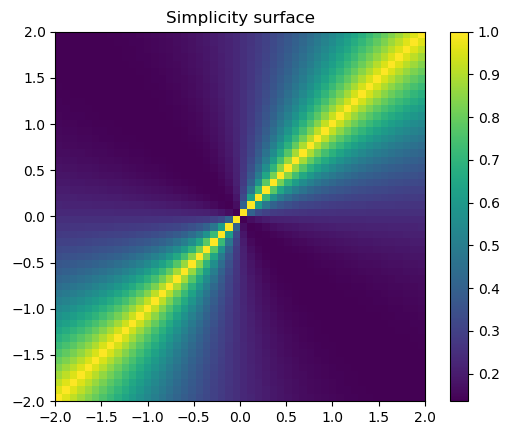
\includegraphics[width=0.8\textwidth,height=0.25\textheight]{../../pictures/figures/complexity_surface_2d-normed.png}
  \label{fig:sub1}
\end{subfigure}%
\begin{subfigure}{.5\textwidth}
  \centering
	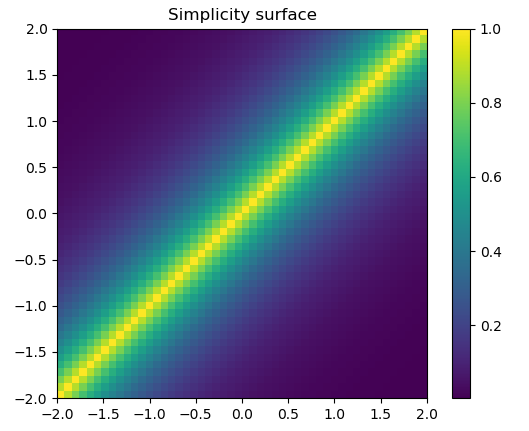
\includegraphics[width=0.8\textwidth,height=0.25\textheight]{../../pictures/figures/complexity_surface_2d-not-normed.png}
  \label{fig:sub2}
\end{subfigure}
\caption{A final decision is about whether we want to normalise the distances,
$\parallel x - P\cdot x \parallel$ (shown on the left), or leave the unnormalised (shown on the right).}
\label{fig:normalise-symmetry}
\end{figure}

A final decision, is whether to normalise the distance measure (see \ref{fig:normalise-symmetry}).
As, we believe the measure of symmetry should be invariant to changes in norm.
For example, if we scale an object by a constant, it should have the same measure of symmetry, $S(10 \cdot x) = S(x)$.

\begin{figure}[h!]
\centering
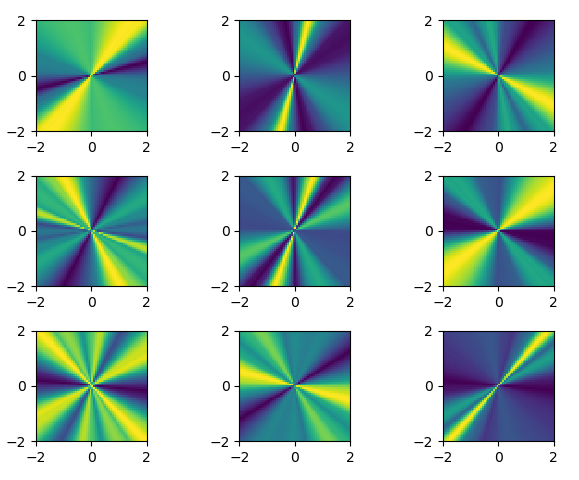
\includegraphics[width=0.7\textwidth,height=0.35\textheight]{../../pictures/figures/complexity_surface_nd-8d.png}
\caption{A visualisation of our measure of symmetry applied to eight dimensional vectors.
We have randomly picked linear projections from the eight dimensions, to two dimensions.
Each pixel represents a vector in the 8D space. Lighter color is more symmetric.}
\label{fig:symmetry-topology}
\end{figure}

\newpage
\mbox{}
\newpage
\subsubsection{Symmetric Rejection Sampling}\label{rejection-sampling}

\begin{displayquote}
	\textit{How can we use this measure of symmetry as a prior?}
\end{displayquote}

We can use rejection sampling to bias produce distributions biased towards symmetric
samples, or in other words, we can use rejection sampling to incorporate our symmetric prior. Let's see how.

\paragraph{Rejection sampling} allows you to generate samples from a target distribution, $p(\cdot)$ (which we cannot efficiently sample from) and a 'related' distribution that we can easily sample from, $q(\cdot)$.
The notion of relatedness of $p(\cdot)$ and $q(\cdot)$ is captured by $k = \mathop{\text{max}}_x \frac{p(x)}{q(x)}$.
This value, $k$ tells us, the average number of rejections before accepting a sample.
Thus, to closely related distributions will have $k\sim 1$. \cite{W.R.1992, Owen2013}

\begin{algorithm}
	\caption{Rejection sampling}
	\begin{algorithmic}[1]

		\Procedure{RS}{$p, q, k$}
		\State $t=0$
		\While{not accepted}
			\State $x\sim U([0, 1])$
			\If{$x < \frac{p(x)}{kq(x)}$}
				\State $Break$
			\EndIf
			\State $t += 1$
		\EndWhile
		\State \algorithmicreturn{ $x$}
		\EndProcedure

	\end{algorithmic}
\end{algorithm}

\paragraph{Incorporating a prior:} We might have some belief over parameters values $\theta$, given some data, $D_t$, which we write as $p(\theta| D_t)$ (the posterior).
We might also have a prior about likely parameter values, in this case, our belief that they should be symmetric $P_{\text{sym}}(\theta)$. Therefore, we can construct the 'target' distribution using Bayes rule.

\begin{align*}
q(\theta | D_t) = \frac{p(D_t | \theta)P_{\text{sym}}(\theta)}{p(D_t)}
\end{align*}

Thus we have a distribution over parameters, $q(\theta | D_t)$, which we can optimise using maximum a posteriori.

Fortunately, we don't need to construct $P_{\text{sym}}(\theta)$, we only need an unnormalised function that it is proportional to \cite{Owen2013}. Meaning, we can use our measure of symmetry $P_{\text{sym}}(\theta)\to S(x)$.

Consider an example: we might have some estimate of a parameter's value, $\mu, \sigma$, which follows a Gaussian distribution $p(\cdot)$. But, we believe the parameters should be symmetric. Therefore, we can construct a new distribution, $q(x | D_t) = p(\mu, \sigma| x)S(x)$. We can use rejection sampling to generate samples from $q(x | D_t)$. See the results below.


\begin{figure}[h!]
  \centering
  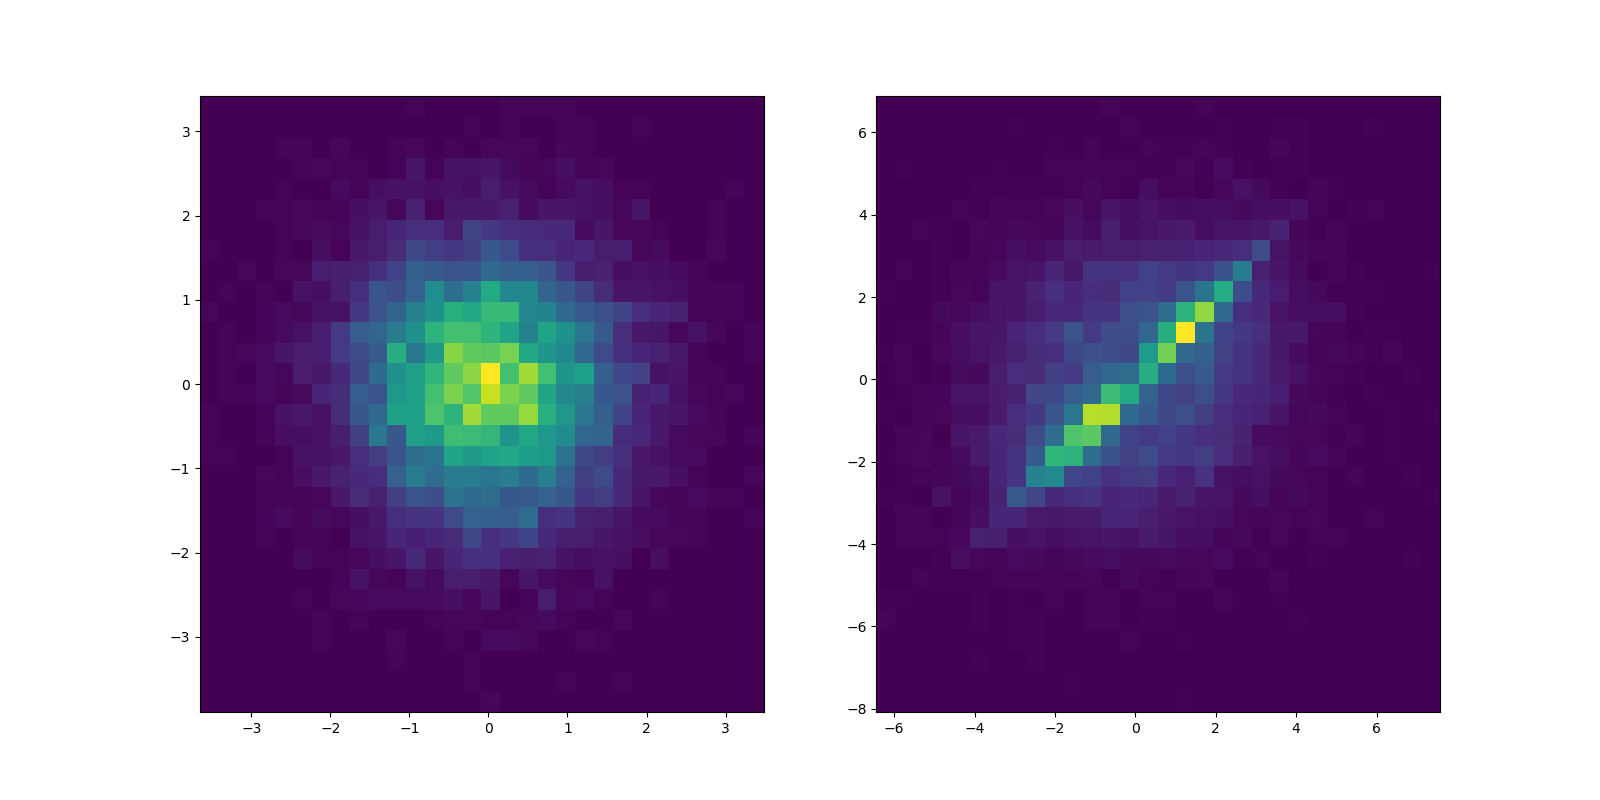
\includegraphics[width=0.8\textwidth,height=0.175\textheight]{../../pictures/figures/symmetric-gaussian.png}
  \caption{On the left we can see a Gaussian distribution of mean zero and variance one, $q(x)$.
  On the right, we have used rejection sampling generate samples from our symmetry biased distribution, $p(x)$.}
\end{figure}

\begin{figure}[h!]
  \centering
  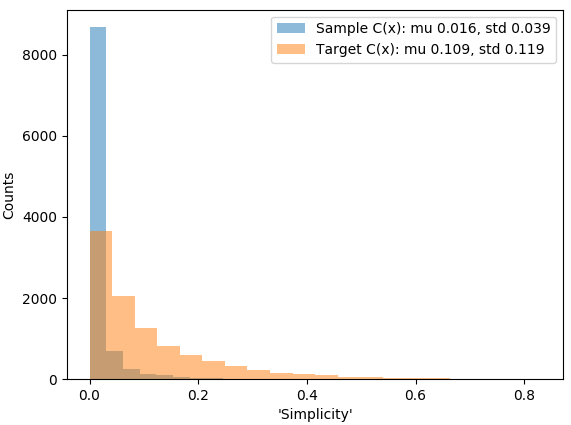
\includegraphics[width=0.5\textwidth,height=0.25\textheight]{../../pictures/figures/s2-prior-rejection-8d.png}
  \caption{Here we have samples from the 'sample distribution', $q(x)$, and the 'target distribution', $p(x)$.
	We can see that the rejection sampling with the symmetry augmented target distribution was successful in producing, on average, more symmetric samples. }
\end{figure}

These results only confirm that we have implemented
rejection sampling correctly, and it works as described.

% \begin{figure}[h!]
% \centering
% 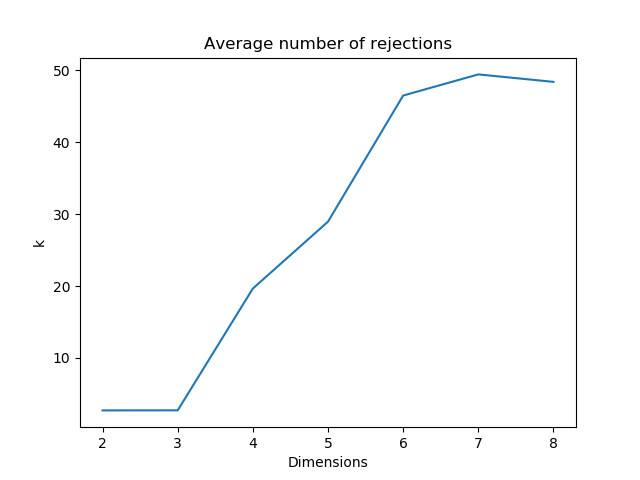
\includegraphics[width=1\textwidth,height=0.5\textheight]{../../pictures/figures/ks.png}
% \caption{}
% \end{figure}

% \subsubsection{Computational issues}
%
% In theory, we can use this approach to bias any distribution of our choice to be more symmetric.
% However, the more different the distributions, the higher the computational costs.
%
% Most general way of adding a prior!?!?
% Doesnt assume that SGD is being done, or some parameterisation... !??!?!
% Because of that, it's also expensive...

\newpage
\subsection{Biased Thompson Sampling} \label{thompson-sampling}

\begin{displayquote}
\textsl{We have a way to apply a symmetric prior to a distribution.
How can we use that to make RL more efficient?}
\end{displayquote}

Here we consider how to use a symmetric prior to make Thompson sampling more sample efficient\footnotemark.

\footnotetext{For a more general picture of the combination of symmetry and RL see \ref{mdp-homomorphism}.}

\subsubsection{Thompson sampling} \label{ts}
\begin{displayquote}
	\textsl{What is Thompson Sampling?}
\end{displayquote}

\begin{displayquote}
	\textit{Thompson sampling is an algorithm for online decision problems where actions are taken sequentially in a manner that
must balance between exploiting what is known to maximize immediate performance and investing to accumulate
new information that may improve future performance.}\cite{Russo2017}
\end{displayquote}

Less cryptically, Thompson sampling estimates the model, $P\, r$. We then act optimally with respect to the estimated model. However, the estimate uncertainty, so ...? We can write this as follows.

\begin{algorithm}
	\caption{Thompson Sampling}
	\begin{algorithmic}[1]

		\Procedure{TS}{$\gamma$}
		\State $t=0$
		\While{not converged}
		\State $(s, a, r, s')$ \Comment{Observe}
		\State $H_t \leftarrow (s, a, r, s', a')$ \Comment{Update history}
		\State $\tau, r \sim P(\cdot | H_t)$ \Comment{Sample a model}
		\State $Q_{t+1}(s, a) = r(s, a) + \gamma \tau(s'| s, a) Q_t(s', a')$ \Comment{Bellman operator}
		\State $\pi_t = \text{greedy}(Q_{t+1})$ \Comment{Act greedily}
		\State $t += 1$

		\EndWhile
		\State \algorithmicreturn{ $\pi_t$}
		\EndProcedure

	\end{algorithmic}
\end{algorithm}

Where $H_t$ is the history of observations, $\{(s_i, a_i, r_i, s_i') : \forall i \in [0, t]\}$.
Further, we construct the estimate of the model as independent distributions of the transition and reward functions $P(\tau, r | H_t) = P(\tau | H_t) \cdot P(r | H_t)$. Where $P(\tau | H_t)$
is modelled as the normalised state transition counts.
And $P(r | H_t)$ is modelled as a isotropic Gaussian.
These can be estimated by storing state-action-state transition counts
and the incremental mean and variance of the rewards.

Note that we act greedily with respect to the $Q$ function. Normally, this would
lead to sub optimal behaviour, because no exploration is being done. But, Thompson sampling
directs exploration through its uncertainty in the model, $\tau, r$. Thus,
exploration occurs by acting greedily with respect to a sampled model.

% \subsubsection{Abstracted Thompson Sampling}
%
% There may be structure in the model,
% Thompson sampling from estimates of similarity / symmetry.
%
% The likelihood of an abstraction, $\tau(A|H_t)$, is modelled as a isotropic (actually should really use full covar?!?!) guassian.
%
% \begin{align*}
% 	\tau(A|H_t) &= \mathcal N(\chi_{\mu}, \chi_{\sigma}) \\
% 	\chi_{\mu} &= \frac{1}{t}\sum_{i=0}^t Q_i \tag{mean} \\
% 	\chi_{\sigma} &= \sqrt{\sum_{i=0}^t (Q_i - \chi_{\mu})^2} \tag{standard deviation}
% \end{align*}
%
% When notice that two states are similar, we group them together. After grouping them, we can apply the Bellman optimality operator.
%
% \begin{algorithm}
% 	\caption{Abstracted Thompson sampling}
% 	\begin{algorithmic}[1]
%
% 		\Procedure{ATS}{$\gamma$}
% 		\State $t=0$
% 		\While{not converged}
% 		\State $(s, a, r, s')$ \Comment{Observe}
% 		\State $H_t \leftarrow (s, a, r, s', a')$ \Comment{Update history}
% 		\State $\tau, R \sim \tau(\cdot | H_t)$ \Comment{Sample a model}
% 		\State $A \sim \tau(\cdot | H_t)$ \Comment{Sample a state abstraction}
% 		\State $\tilde \tau, \tilde r, \tilde Q_t = A(\tau, r, Q_t)$ \Comment{Do a model reduction}
% 		\State $\tilde Q_{t+1}(s, a) = \tilde r(s, a) + \gamma \tilde \tau(s'| s, a) \tilde Q_t(s', a')$ \Comment{Bellman operator}
% 		\State $Q_{t+1} = S^{-1}(\tilde Q_{t+1})$ \Comment{Lift the values}
% 		\State $\pi_t = \text{greedy}(Q_{t+1})$ \Comment{Act greedily}
% 		\State $t += 1$
%
% 		\EndWhile
% 		\State \algorithmicreturn{ $\pi_t$}
% 		\EndProcedure
%
% 	\end{algorithmic}
% \end{algorithm}
%
% % if we were certain enough, we could throw away estimates of certain states. and just work in the abstracted domain?!
%
% This doesnt really work. For a few reasons. Costs a lot of keep track of the pairwise state similarities.
% Saves compute on Bellman step.
% But overall, is costs more compute than has been gained.
%
% Shouldn't effect sample efficiency. (unless we replace the tabular model with something that can generalise)

\subsubsection{Biased Thompson Sampling}\label{bts}

\begin{displayquote}
\textsl{Given uncertainty, prefer symmetry}
\end{displayquote}

The difference between \textit{Thompson Sampling} and \textit{Biased Thompson Sampling}
is how we construct the distribution over models, $P(\tau, r |D)$.

We believe that the states will have group structure, a symmetry.
We use the symmetric rejection sampling method, outlined above (\ref{rejection-sampling}) to bias the
distribution over models towards more symmetric models.

To simplify, we estimate $P_{\text{sym}}(\tau, R)$ as $P_{\text{sym}}(R)$. That is, we believe there will be symmetries in the reward function, not necessarily in the transition function.

% \subsubsection{Biased Abstracted Thompson Sampling}
%
% Similarly, we can apply the same idea to \textit{Abstracted Thompson Sampling}.
% We can use the prior: state abstractions, $A$, that are symmetric should be more likely.
%
% To achieve this, we need to construct a distribution, $P_S(A)$, that prefers more symmetric abstractions.
% We can then use this prior, with maximum a posterori, to estimate the posteror as $\tau(A | H_t) = \frac{\tau(H_t | A)P_S(A)}{\tau(H_t)}$.

\subsubsection{Experiments}

% \begin{displayquote}
% 	\textsl{Sounds good in theory. Does it work in practice?}
% \end{displayquote}

We want to demonstrate that Biased Thompson Sampling \ref{bts} has greater sample efficiency (when applied to problems with a symmetry present) than Thompson Sampling \ref{ts}.
And therefore that this learner can exploit symmetries present in a RL problem\footnotemark.

\footnotetext{Note, we explore another, more complicated, setting to test a learners ability to exploit symmetries in \ref{action-space-experiments}.}
% There are a few factors that could effect the (potential) advangate of Biased Thompson Sampling.
We ran experiments with symmetric n-armed bandit problems, and symmetric grid worlds \ref{race-grid-world}, the results are shown in figures \ref{fig:map-bts} and \ref{fig:explicit-sym}.


% Explicit symmetry prior versus 'high level' prior.

% Despite, intuition, we have been unable to show that Biased Thompson Sampling probides any advantage. We leave this for future work.

% \begin{figure}[h!]
%   \centering
%   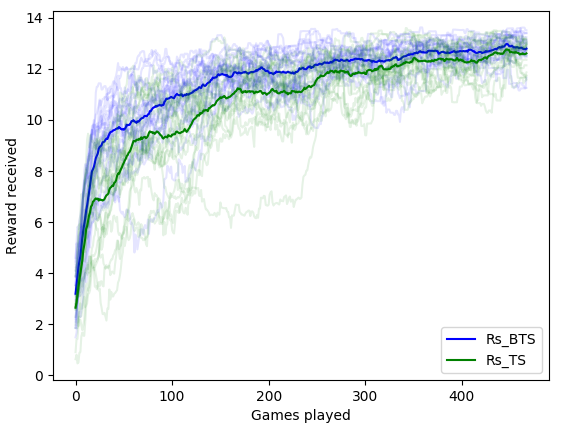
\includegraphics[width=0.7\textwidth,height=0.35\textheight]{../../pictures/figures/mab-9-ts.png}
%   \caption{A 8 armed bandit problem, with means and variances chosen randomly.
% 	We can see that Biased Thompson sampling does not perform better in any significant sense.}
% \end{figure}

\begin{figure}[h!]
  \centering
  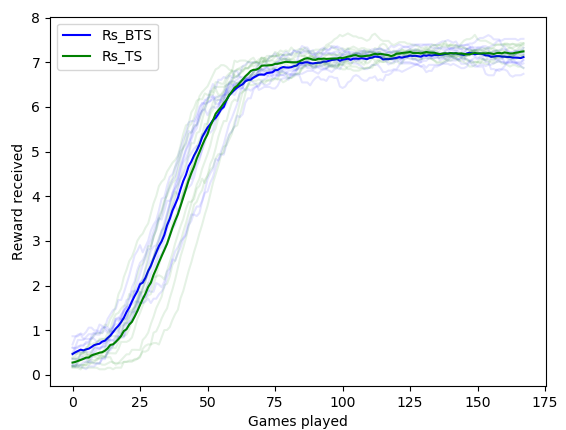
\includegraphics[width=0.6\textwidth,height=0.3\textheight]{../../pictures/figures/mdp-9-implicit.png}
  \caption{A 9 state symmetric grid world problem.
	We can see that Biased Thompson sampling, using our symmetry measure, does not perform better than Thompson sampling in any significant sense.}
	\label{fig:map-bts}
\end{figure}

\begin{figure}[h!]
  \centering
  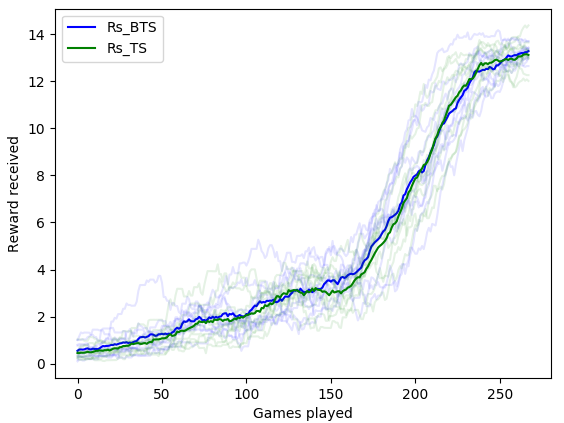
\includegraphics[width=0.6\textwidth,height=0.3\textheight]{../../pictures/figures/mdp-25-explicit.png}
  \caption{A 25 state symmetric grid world problem.
	This Biased Thompson Sampler was given explicit knowledge of the underlying symmetry.
	Despite this, we can see that Biased Thompson sampling does not perform better in any significant sense.}
	\label{fig:explicit-sym}
\end{figure}

% \begin{center}\rule{0.5\linewidth}{\linethickness}\end{center}

% Of course, the symmetry didn't need to be inferred. So it's cheating.
% We could have simply built the symmetry into the solver. But we want to
% construct a 'high' level prior that is not specific to a single problem (like $S_2$ is), but
% to many. Something that prefers symmetries of any kind.

These figures show that Biased Thompson Sampling provides no advantage in sample efficiency (while using a lot more compute).
However, we cannot conclude that Biased Thompson Sampling provides no advantage. This is because we also tested a Biased Thompson Sampler given explicit knowledge of the symmetry within a MDP,
and it, also, did not show any advantage (see \ref{fig:explicit-sym}). This result tell us that our method of biasing a distribution over models (via rejection sampling)
does not seem to help RL. It says nothing about the utility of similarity measure.

Also, we expect the advantage should become clearer as we scale to larger state spaces (as there is more benefit to symmetry, there are more similar states).
However, we were unable to scale to larger problems due to the computational complexity of building the family of symmetries (see \ref{implementation-issues}).
